% Minimum Spanning Trees -- Metropolis beamer slides
% Compile: pdflatex minimum-spanning-tree.tex (x2)
\documentclass[10pt,aspectratio=169]{beamer}

\usetheme{metropolis}
\metroset{block=fill, numbering=fraction, progressbar=frametitle}

\usepackage[T1]{fontenc}
\usepackage{amsmath, amssymb}
\usepackage{listings}
\usepackage{booktabs}
\usepackage{tikz}
\usetikzlibrary{arrows.meta, positioning, calc, decorations.pathmorphing}

% ---- colors -------------------------------------------------------------
\definecolor{mLightBlue}{HTML}{4C72B0}
\definecolor{mGreen}{HTML}{55A868}
\definecolor{mRed}{HTML}{C44E52}
\definecolor{mGray}{HTML}{BFBFBF}
\definecolor{mOrange}{HTML}{DD8452}
\setbeamercolor{alerted text}{fg=mRed}

% ---- code style ---------------------------------------------------------
\lstdefinestyle{jl}{
  basicstyle=\ttfamily\footnotesize,
  keywordstyle=\color{mRed}\bfseries,
  commentstyle=\color{mGreen}\itshape,
  numberstyle=\tiny\color{mGray},
  showstringspaces=false,
  breaklines=true,
  columns=fullflexible,
  morekeywords={function,for,in,if,else,elseif,end,return,length,while,continue,break,using}
}
\lstset{style=jl}

% ---- graph helpers ------------------------------------------------------
\tikzset{
  vtx/.style={draw, circle, minimum size=7mm, inner sep=0pt, font=\small,
              fill=white},
  edg/.style={thick, mGray!80!black},
  wlbl/.style={fill=white, inner sep=1.5pt, font=\scriptsize, text=black},
  tree/.style={line width=2.2pt, mLightBlue},
  cand/.style={line width=1.4pt, mOrange, dashed},
  pick/.style={line width=2.2pt, mRed},
  rej/.style={mGray, dotted},
  intree/.style={fill=mLightBlue!30},
  % overlay-aware keys: onslide=<2->{tree}
  onslide/.code args={<#1>#2}{\only<#1>{\pgfkeysalso{#2}}},
}

% Vertex positions of the running example
\newcommand{\mstnodes}[6]{%
  \node[vtx, #1] (a) at (0,1)      {$a$};
  \node[vtx, #2] (b) at (2,2.3)    {$b$};
  \node[vtx, #3] (c) at (4.6,2.3)  {$c$};
  \node[vtx, #4] (d) at (6.6,1)    {$d$};
  \node[vtx, #5] (e) at (2,-0.3)   {$e$};
  \node[vtx, #6] (f) at (4.6,-0.3) {$f$};
}

% ---- title --------------------------------------------------------------
\title{Minimum Spanning Trees}
\subtitle{The Cut Property, Prim's Algorithm, Kruskal's Algorithm}
\date{}
\author{}

\begin{document}

\maketitle

% =========================================================================
\begin{frame}{The Problem}
  Let $G = (V, E)$ be a \alert{connected, undirected} graph with edge weights
  $w(e)$.

  \begin{itemize}
    \item A \alert{spanning tree} is a subset $T \subseteq E$ that connects
          all vertices and has no cycle.
    \item Its weight is $w(T) = \sum_{e \in T} w(e)$.
    \item A \alert{minimum spanning tree} (MST) has the smallest weight among
          all spanning trees.
  \end{itemize}

  \begin{center}
  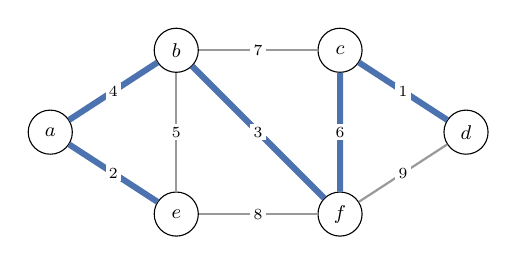
\begin{tikzpicture}[scale=0.8, every node/.append style={transform shape}]
    \mstnodes{}{}{}{}{}{}
    \draw[edg] (a) -- node[wlbl] {4} (b);
    \draw[edg] (b) -- node[wlbl] {5} (e);
    \draw[edg] (b) -- node[wlbl] {7} (c);
    \draw[edg] (e) -- node[wlbl] {8} (f);
    \draw[edg] (f) -- node[wlbl] {9} (d);
    \draw[edg] (a) -- node[wlbl] {2} (e);
    \draw[edg] (b) -- node[wlbl] {3} (f);
    \draw[edg] (c) -- node[wlbl] {6} (f);
    \draw[edg] (c) -- node[wlbl] {1} (d);
    \onslide<2->{
      \draw[tree] (a) -- (b); \draw[tree] (a) -- (e); \draw[tree] (b) -- (f);
      \draw[tree] (c) -- (f); \draw[tree] (c) -- (d);
      \node[wlbl] at ($(a)!0.5!(b)$) {4}; \node[wlbl] at ($(a)!0.5!(e)$) {2};
      \node[wlbl] at ($(b)!0.5!(f)$) {3}; \node[wlbl] at ($(c)!0.5!(f)$) {6};
      \node[wlbl] at ($(c)!0.5!(d)$) {1};
    }
  \end{tikzpicture}
  \end{center}

  \onslide<2->{\begin{center}
    The MST (blue) has weight $2 + 4 + 3 + 6 + 1 = 16$.
  \end{center}}
\end{frame}

\begin{frame}{Facts About Trees}
  For a graph on $n$ vertices:

  \begin{itemize}
    \item Every spanning tree has exactly $n - 1$ edges.
    \item Adding any edge to a spanning tree creates \alert{exactly one}
          cycle.
    \item Removing any edge of that cycle gives a spanning tree again.
  \end{itemize}

  \begin{center}
  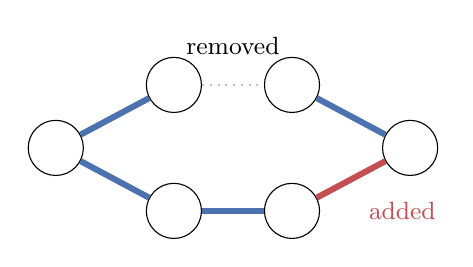
\begin{tikzpicture}
    \node[vtx] (1) at (0,0) {};   \node[vtx] (2) at (1.5,0.8) {};
    \node[vtx] (3) at (3,0.8) {}; \node[vtx] (4) at (4.5,0) {};
    \node[vtx] (5) at (1.5,-0.8) {}; \node[vtx] (6) at (3,-0.8) {};
    \draw[tree] (1) -- (2); \draw[tree] (2) -- (3); \draw[tree] (3) -- (4);
    \draw[tree] (1) -- (5); \draw[tree] (5) -- (6);
    \onslide<2->{\draw[pick] (6) -- (4);
      \node[mRed, font=\small] at (4.4,-0.8) {added};}
    \onslide<3->{\draw[line width=2.2pt, white] (2) -- (3);
      \draw[rej, thick] (2) -- (3);
      \node[font=\small] at (2.25,1.3) {removed};}
  \end{tikzpicture}
  \end{center}

  \onslide<3->{This swap is the main tool in every MST proof.}
\end{frame}

\begin{frame}{Applications}
  \begin{itemize}
    \item \textbf{Network design.} Connect cities, offices, or circuit pins
          with cables, pipes, or roads as cheaply as possible.
    \item \textbf{Clustering.} Build an MST of the data points and delete its
          $k - 1$ heaviest edges: the $k$ remaining pieces are the
          single-linkage clusters.
    \item \textbf{Approximation.} An MST gives a tour at most twice the
          optimum for the metric travelling salesman problem.
    \item \textbf{Image segmentation.} Pixels are vertices, edge weights are
          colour differences; MST-based methods split the image into regions.
    \item \textbf{Bottleneck paths.} The path between $u$ and $v$ in an MST
          minimises the heaviest edge used.
  \end{itemize}

  \bigskip
  \small Throughout, we assume all edge weights are \alert{distinct}. Then the
  MST is unique, which makes the proofs cleaner. Everything still works with
  ties, broken consistently.
\end{frame}

% =========================================================================
\section{The Cut Property}

\begin{frame}{Cuts}
  A \alert{cut} is a partition of the vertices into $S$ and $V \setminus S$,
  both nonempty. An edge \alert{crosses} the cut if it has one endpoint on
  each side.

  \begin{center}
  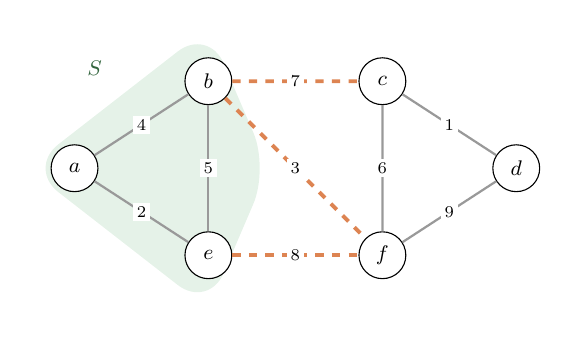
\begin{tikzpicture}[scale=0.85, every node/.append style={transform shape}]
    \fill[mGreen!15, rounded corners=14pt]
      (-0.7,1) -- (2,3.1) -- (2.9,1) -- (2,-1.1) -- cycle;
    \node[mGreen!60!black, font=\small] at (0.3,2.5) {$S$};
    \mstnodes{}{}{}{}{}{}
    \draw[edg] (a) -- node[wlbl] {4} (b);
    \draw[edg] (b) -- node[wlbl] {5} (e);
    \draw[edg] (a) -- node[wlbl] {2} (e);
    \draw[edg] (f) -- node[wlbl] {9} (d);
    \draw[edg] (c) -- node[wlbl] {6} (f);
    \draw[edg] (c) -- node[wlbl] {1} (d);
    \draw[cand] (b) -- node[wlbl] {7} (c);
    \draw[cand] (e) -- node[wlbl] {8} (f);
    \draw[cand, onslide=<2->{pick, solid}] (b) -- node[wlbl] {3} (f);
  \end{tikzpicture}
  \end{center}

  Here $S = \{a, b, e\}$. The crossing edges (orange) have weights
  $7, 3, 8$. \onslide<2->{The \alert{lightest} crossing edge is $b$--$f$.}
\end{frame}

\begin{frame}{The Cut Property}
  \begin{block}{Cut property}
    For any cut $(S, V \setminus S)$, the lightest edge crossing the cut
    belongs to the MST.
  \end{block}

  \bigskip
  \textbf{Proof} (exchange). Let $e = \{u, v\}$ be the lightest crossing edge,
  $u \in S$, and suppose the MST $T$ does not contain $e$.

  \begin{columns}[c]
    \begin{column}{0.45\textwidth}
      \begin{center}
      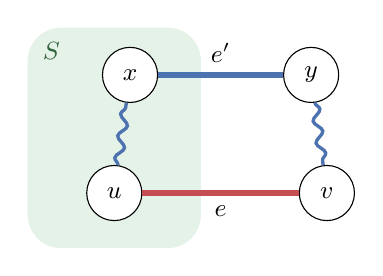
\begin{tikzpicture}
        \fill[mGreen!15, rounded corners=12pt] (-0.6,-1.4) rectangle (1.6,1.4);
        \node[mGreen!60!black, font=\small] at (-0.3,1.1) {$S$};
        \node[vtx] (u) at (0.5,-0.7) {$u$};
        \node[vtx] (v) at (3.2,-0.7) {$v$};
        \node[vtx] (x) at (0.7,0.8) {$x$};
        \node[vtx] (y) at (3,0.8) {$y$};
        \draw[very thick, mLightBlue, decorate,
              decoration={snake, amplitude=1.5pt, segment length=8pt}] (u) -- (x);
        \draw[very thick, mLightBlue, decorate,
              decoration={snake, amplitude=1.5pt, segment length=8pt}] (y) -- (v);
        \draw[tree, onslide=<3->{rej, line width=1pt}] (x) -- node[above, font=\small,
              text=black] {$e'$} (y);
        \draw[pick, onslide=<1>{dashed}] (u) -- node[below, font=\small,
              text=black] {$e$} (v);
      \end{tikzpicture}
      \end{center}
    \end{column}
    \begin{column}{0.52\textwidth}
      \begin{itemize}
        \item<2-> The path from $u$ to $v$ in $T$ starts in $S$ and ends
              outside, so it uses some crossing edge $e' = \{x, y\}$.
        \item<3-> $T' = T - e' + e$ is a spanning tree (swap on the cycle
              formed by $e$).
        \item<4-> $w(e) < w(e')$, so $w(T') < w(T)$. Contradiction.
              \hfill $\square$
      \end{itemize}
    \end{column}
  \end{columns}
\end{frame}

\begin{frame}{A Generic Greedy Algorithm}
  The cut property gives a recipe for building the MST one edge at a time.

  \begin{block}{Generic MST}
    Start with $F = \emptyset$. Repeat $n - 1$ times:
    \begin{enumerate}
      \item choose a cut that \alert{no edge of $F$ crosses},
      \item add the lightest edge crossing it to $F$.
    \end{enumerate}
  \end{block}

  \begin{itemize}
    \item Every added edge is in the MST, by the cut property.
    \item The chosen cut separates two different pieces of $F$, so no cycle
          is ever created.
  \end{itemize}

  \pause
  \medskip
  Prim and Kruskal are two ways of choosing the cut:
  \begin{itemize}
    \item \textbf{Prim}: $S$ = the vertices of the single tree grown so far.
    \item \textbf{Kruskal}: $S$ = the component of one endpoint of the next
          lightest useful edge.
  \end{itemize}
\end{frame}

% =========================================================================
\section{Prim's Algorithm}

\begin{frame}{Prim's Algorithm}
  Grow a single tree from a start vertex $s$.

  \begin{block}{Prim}
    $S = \{s\}$, $T = \emptyset$. While $S \ne V$: add the lightest edge
    $\{u, v\}$ with $u \in S$, $v \notin S$ to $T$, and add $v$ to $S$.
  \end{block}

  \bigskip
  \begin{itemize}
    \item Each step uses the cut $(S, V \setminus S)$. No edge of $T$ crosses
          it, so the cut property says the new edge is in the MST.
    \item After $n - 1$ steps, $T$ is a spanning tree made of MST edges: it is
          the MST.
  \end{itemize}

  \bigskip
  It looks just like Dijkstra, except the priority of $v$ is the weight of
  the \alert{single edge} into $S$, not the distance from $s$.
\end{frame}

\begin{frame}{Prim in Action (start at $a$)}
  \begin{columns}[c]
    \begin{column}{0.58\textwidth}
      \begin{center}
      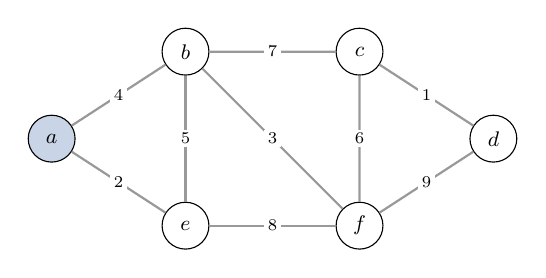
\begin{tikzpicture}[scale=0.85, every node/.append style={transform shape}]
        \mstnodes{intree}{onslide=<3->{intree}}{onslide=<5->{intree}}%
                 {onslide=<6->{intree}}{onslide=<2->{intree}}%
                 {onslide=<4->{intree}}
        \draw[edg, onslide=<1>{pick}, onslide=<2->{tree}]
          (a) -- node[wlbl] {2} (e);
        \draw[edg, onslide=<1>{cand}, onslide=<2>{pick}, onslide=<3->{tree}]
          (a) -- node[wlbl] {4} (b);
        \draw[edg, onslide=<2>{cand}] (b) -- node[wlbl] {5} (e);
        \draw[edg, onslide=<2-3>{cand}] (e) -- node[wlbl] {8} (f);
        \draw[edg, onslide=<3>{pick}, onslide=<4->{tree}]
          (b) -- node[wlbl] {3} (f);
        \draw[edg, onslide=<3-4>{cand}] (b) -- node[wlbl] {7} (c);
        \draw[edg, onslide=<4>{pick}, onslide=<5->{tree}]
          (c) -- node[wlbl] {6} (f);
        \draw[edg, onslide=<4-5>{cand}] (f) -- node[wlbl] {9} (d);
        \draw[edg, onslide=<5>{pick}, onslide=<6->{tree}]
          (c) -- node[wlbl] {1} (d);
      \end{tikzpicture}
      \end{center}
    \end{column}
    \begin{column}{0.4\textwidth}
      \small
      \only<1>{$S = \{a\}$. Crossing: $4, 2$.\\ Add $a$--$e$ (2).}%
      \only<2>{$S = \{a, e\}$. Crossing: $4, 5, 8$.\\ Add $a$--$b$ (4).}%
      \only<3>{$S = \{a, b, e\}$. Crossing: $3, 7, 8$.\\ Add $b$--$f$ (3).}%
      \only<4>{$S = \{a, b, e, f\}$. Crossing: $7, 6, 9$.\\
               Add $c$--$f$ (6).}%
      \only<5>{$S = \{a, b, c, e, f\}$. Crossing: $1, 9$.\\
               Add $c$--$d$ (1).}%
      \only<6>{$S = V$. Done.\\ Weight $2 + 4 + 3 + 6 + 1 = 16$.}

      \bigskip
      \textcolor{mOrange}{dashed}: crossing the cut\\
      \textcolor{mRed}{red}: lightest crossing edge\\
      \textcolor{mLightBlue}{blue}: tree so far
    \end{column}
  \end{columns}
\end{frame}

\begin{frame}{Implementing Prim}
  For each $v \notin S$ keep
  \[
    \text{key}[v] = \text{weight of the lightest edge from } S \text{ to } v
    \quad (\infty \text{ if none}),
  \]
  in a min-priority queue, together with $\text{parent}[v]$, the other end
  of that edge.

  \bigskip
  \begin{enumerate}
    \item Extract the $v$ with smallest key; add $v$ and
          $\{\text{parent}[v], v\}$ to the tree.
    \item For each neighbour $x \notin S$ of $v$: if $w(v, x) < \text{key}[x]$,
          set $\text{key}[x] = w(v, x)$, $\text{parent}[x] = v$.
  \end{enumerate}

  \bigskip
  \begin{center}
  \begin{tabular}{lc}
    \toprule
    priority queue & time \\
    \midrule
    array, linear scan & $O(n^2)$ \hfill dense graphs \\
    binary heap & $O((n + m) \log n)$ \\
    \bottomrule
  \end{tabular}
  \end{center}
\end{frame}

\begin{frame}[fragile]{Prim in Julia}
\begin{lstlisting}[basicstyle=\ttfamily\scriptsize]
using DataStructures: PriorityQueue, dequeue_pair!

function prim(n, adj, s = 1)        # adj[u]: list of (v, weight) pairs
    key, parent, intree = fill(Inf, n), zeros(Int, n), falses(n)
    key[s] = 0.0
    pq = PriorityQueue{Int, Float64}(s => 0.0)
    while !isempty(pq)
        u, _ = dequeue_pair!(pq)
        intree[u] = true
        for (v, w) in adj[u]
            if !intree[v] && w < key[v]   # lighter edge from the tree to v
                key[v]    = w
                parent[v] = u
                pq[v] = w                 # insert, or lower its key
            end
        end
    end
    return parent   # MST edges: (parent[v], v) for every v != s
end
\end{lstlisting}
\end{frame}

% =========================================================================
\section{Kruskal's Algorithm}

\begin{frame}{Kruskal's Algorithm}
  Consider the edges from lightest to heaviest.

  \begin{block}{Kruskal}
    Sort the edges by weight. For each edge $\{u, v\}$ in order: if $u$ and
    $v$ are in different components of $T$, add the edge to $T$; otherwise
    skip it (it would close a cycle).
  \end{block}

  \bigskip
  \begin{itemize}
    \item $T$ is a forest that slowly merges into one tree.
    \item ``Are $u$ and $v$ in the same component?'' and ``merge the two
          components'' are exactly \texttt{find} and \texttt{union}:
          use \alert{union-find}.
  \end{itemize}
\end{frame}

\begin{frame}{Kruskal in Action}
  \begin{columns}[c]
    \begin{column}{0.58\textwidth}
      \begin{center}
      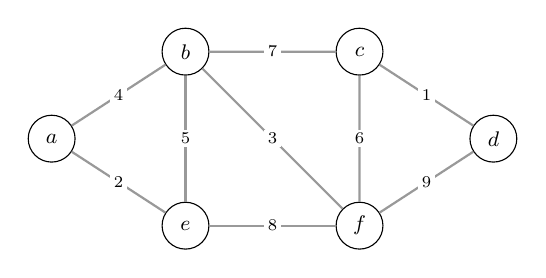
\begin{tikzpicture}[scale=0.85, every node/.append style={transform shape}]
        \mstnodes{}{}{}{}{}{}
        \draw[edg, onslide=<2>{pick}, onslide=<3->{tree}]
          (c) -- node[wlbl] {1} (d);
        \draw[edg, onslide=<3>{pick}, onslide=<4->{tree}]
          (a) -- node[wlbl] {2} (e);
        \draw[edg, onslide=<4>{pick}, onslide=<5->{tree}]
          (b) -- node[wlbl] {3} (f);
        \draw[edg, onslide=<5>{pick}, onslide=<6->{tree}]
          (a) -- node[wlbl] {4} (b);
        \draw[edg, onslide=<6>{cand}, onslide=<7->{rej}]
          (b) -- node[wlbl] {5} (e);
        \draw[edg, onslide=<7>{pick}, onslide=<8->{tree}]
          (c) -- node[wlbl] {6} (f);
        \draw[edg, onslide=<8>{cand}, onslide=<9->{rej}]
          (b) -- node[wlbl] {7} (c);
        \draw[edg, onslide=<9>{cand}, onslide=<10->{rej}]
          (e) -- node[wlbl] {8} (f);
        \draw[edg, onslide=<10>{cand}, onslide=<11->{rej}]
          (f) -- node[wlbl] {9} (d);
      \end{tikzpicture}
      \end{center}
    \end{column}
    \begin{column}{0.4\textwidth}
      \small
      \begin{tabular}{lcl}
        edge & $w$ & \\ \midrule
        $c$--$d$ & 1 & \onslide<2->{add} \\
        $a$--$e$ & 2 & \onslide<3->{add} \\
        $b$--$f$ & 3 & \onslide<4->{add} \\
        $a$--$b$ & 4 & \onslide<5->{add} \\
        $b$--$e$ & 5 & \onslide<6->{\textcolor{mOrange}{skip}: $b, e$ joined} \\
        $c$--$f$ & 6 & \onslide<7->{add} \\
        $b$--$c$ & 7 & \onslide<8->{\textcolor{mOrange}{skip}: $b, c$ joined} \\
        $e$--$f$ & 8 & \onslide<9->{\textcolor{mOrange}{skip}} \\
        $f$--$d$ & 9 & \onslide<10->{\textcolor{mOrange}{skip}} \\
      \end{tabular}

      \medskip
      \onslide<11->{Same tree as Prim, weight 16.}
    \end{column}
  \end{columns}
\end{frame}

\begin{frame}{Why Kruskal Is Correct}
  Suppose Kruskal adds $e = \{u, v\}$. Let $C$ be the component of $T$
  containing $u$ at that moment, and use the cut $(C, V \setminus C)$.

  \begin{center}
  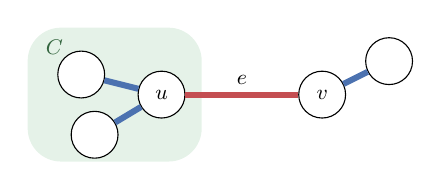
\begin{tikzpicture}[scale=0.85, every node/.append style={transform shape}]
    \fill[mGreen!15, rounded corners=12pt] (-0.8,-1) rectangle (1.8,1);
    \node[mGreen!60!black, font=\small] at (-0.4,0.7) {$C$};
    \node[vtx] (u) at (1.2,0) {$u$};
    \node[vtx] (p) at (0,0.3) {};  \node[vtx] (q) at (0.2,-0.6) {};
    \draw[tree] (p) -- (u); \draw[tree] (q) -- (u);
    \node[vtx] (v) at (3.6,0) {$v$};
    \node[vtx] (r) at (4.6,0.5) {};
    \draw[tree] (v) -- (r);
    \draw[pick] (u) -- node[above, font=\small, text=black] {$e$} (v);
  \end{tikzpicture}
  \end{center}

  \begin{itemize}
    \item No edge of $T$ crosses the cut: $C$ is a whole component.
    \item $v \notin C$, so $e$ crosses the cut.
    \item Every lighter edge was already considered and now lies inside a
          component (it was added, or skipped because its endpoints were
          joined). So $e$ is the \alert{lightest} crossing edge.
  \end{itemize}
  By the cut property $e$ is in the MST; since $G$ is connected, $T$ ends as a
  spanning tree. \hfill $\square$
\end{frame}

\begin{frame}[fragile]{Kruskal in Julia}
  \begin{columns}[c]
    \begin{column}{0.55\textwidth}
\begin{lstlisting}
# edges: list of (weight, u, v)
# UnionFind, union! from the union-find lecture
function kruskal(n, edges)
    uf  = UnionFind(n)
    mst = Tuple{Int, Int, Float64}[]
    for (w, u, v) in sort(edges)
        if union!(uf, u, v)      # different components
            push!(mst, (u, v, w))
        end
    end
    return mst
end
\end{lstlisting}
    \end{column}
    \begin{column}{0.42\textwidth}
      \textbf{Running time}
      \begin{itemize}
        \item Sorting: $O(m \log m) = O(m \log n)$.
        \item $m$ union-find operations: $O(m \, \alpha(n))$.
        \item Total $O(m \log n)$, dominated by the sort.
      \end{itemize}

      \medskip
      If the edges arrive already sorted, Kruskal runs in nearly linear time.
    \end{column}
  \end{columns}
\end{frame}

% =========================================================================
\begin{frame}{Prim vs.\ Kruskal}
  \begin{center}
  \begin{tabular}{lll}
    \toprule
    & Prim & Kruskal \\
    \midrule
    grows & one tree from $s$ & a forest that merges \\
    cut used & tree vs.\ rest & component vs.\ rest \\
    data structure & priority queue & sorting $+$ union-find \\
    time & $O((n + m) \log n)$, or $O(n^2)$ & $O(m \log n)$ \\
    best for & dense graphs (array version) & sparse graphs, sorted edges \\
    \bottomrule
  \end{tabular}
  \end{center}

  \bigskip
  Both are greedy, and both are correct for the same reason: every edge they
  add is the lightest edge across some cut that the current edges do not
  cross.
\end{frame}

% =========================================================================
\begin{frame}{Exercise}
  \begin{columns}[c]
    \begin{column}{0.4\textwidth}
      \begin{center}
      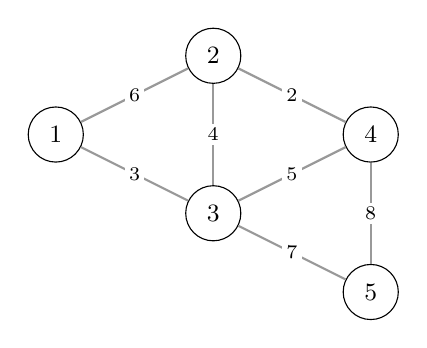
\begin{tikzpicture}
        \node[vtx] (1) at (0,1)    {1};
        \node[vtx] (2) at (2,2)    {2};
        \node[vtx] (3) at (2,0)    {3};
        \node[vtx] (4) at (4,1)    {4};
        \node[vtx] (5) at (4,-1)   {5};
        \draw[edg] (1) -- node[wlbl] {6} (2);
        \draw[edg] (1) -- node[wlbl] {3} (3);
        \draw[edg] (2) -- node[wlbl] {4} (3);
        \draw[edg] (2) -- node[wlbl] {2} (4);
        \draw[edg] (3) -- node[wlbl] {5} (4);
        \draw[edg] (3) -- node[wlbl] {7} (5);
        \draw[edg] (4) -- node[wlbl] {8} (5);
      \end{tikzpicture}
      \end{center}
    \end{column}
    \begin{column}{0.56\textwidth}
      \begin{enumerate}
        \item Run Kruskal. List the edges in the order they are added and the
              edges that are skipped.
        \item Run Prim from vertex 1. List the edges in the order they are
              added.
        \item The weight of edge $3$--$5$ rises from $7$ to $10$. Which edge
              replaces it, and what is the new MST weight?
      \end{enumerate}
    \end{column}
  \end{columns}
\end{frame}

\begin{frame}{Solution}
  \begin{columns}[c]
    \begin{column}{0.4\textwidth}
      \begin{center}
      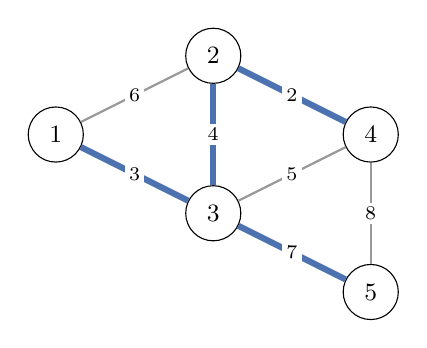
\begin{tikzpicture}
        \node[vtx] (1) at (0,1)    {1};
        \node[vtx] (2) at (2,2)    {2};
        \node[vtx] (3) at (2,0)    {3};
        \node[vtx] (4) at (4,1)    {4};
        \node[vtx] (5) at (4,-1)   {5};
        \draw[edg] (1) -- node[wlbl] {6} (2);
        \draw[tree] (1) -- node[wlbl] {3} (3);
        \draw[tree] (2) -- node[wlbl] {4} (3);
        \draw[tree] (2) -- node[wlbl] {2} (4);
        \draw[edg] (3) -- node[wlbl] {5} (4);
        \draw[tree, onslide=<2->{rej, line width=1pt}] (3) -- node[wlbl] {7} (5);
        \draw[edg, onslide=<2->{tree}] (4) -- node[wlbl] {8} (5);
      \end{tikzpicture}
      \end{center}
    \end{column}
    \begin{column}{0.56\textwidth}
      \small
      \textbf{(a)} Add $2$--$4$ (2), $1$--$3$ (3), $2$--$3$ (4).
      Skip $3$--$4$ (5) and $1$--$2$ (6), whose endpoints are already joined.
      Add $3$--$5$ (7). Skip $4$--$5$ (8).

      \medskip
      \textbf{(b)} $1$--$3$ (3), $2$--$3$ (4), $2$--$4$ (2), $3$--$5$ (7).
      Same tree, weight $16$.

      \pause
      \medskip
      \textbf{(c)} Vertex 5 has only two edges. With $3$--$5$ at $10$, the
      cut $(\{5\}, \text{rest})$ has lightest edge $4$--$5$ (8), so it
      replaces $3$--$5$. New weight $2 + 3 + 4 + 8 = 17$.
    \end{column}
  \end{columns}
\end{frame}

% =========================================================================
\begin{frame}{Summary}
  \begin{itemize}
    \item An MST connects all vertices with the least total weight, using
          $n - 1$ edges.
    \item \alert{Cut property}: the lightest edge across any cut is in the
          MST. Proof: swap it with the tree edge that crosses the cut.
    \item \alert{Prim}: grow one tree, always adding the lightest edge
          leaving it. Priority queue, $O((n + m) \log n)$.
    \item \alert{Kruskal}: scan edges by weight, add those joining two
          components. Sorting plus union-find, $O(m \log n)$.
  \end{itemize}
\end{frame}

\end{document}
